
\chapter{Construcción de modelos}

\section{Representación diagramática de interacciones}

Como un término en el Lagrangiano respeta todas las cargas conservadas,  se puede visualizar en términos de corrientes que fluyen. 
Por ejemplo, si denotamos el doblete de Higgs de hipercarga $1/2$ como
$H$, podemos escribir el término del Lagrangiano con el Higgs, el quark $u_R$ y el doblete de quarks $Q$ como
\begin{align}
  \mathcal{L}_u=h_u \left( u_R \right)^{\dagger} Q H\,. 
\end{align}

El flujo de hipercarga puede visualizarse en la figura~\ref{fig:yg}. Allí la linea a trazos representa a la partícula escalar y las continuas a los fermiones.  Las cargas que entran deben igualar a las cargas que salen en el vértice de la figura donde confluyen los tres campos, correspondiente al punto verde. Denotando por simplicidad la hipercarga con el símbolo del campo, tenemos entonces que
\begin{align}
  \label{eq:urn}
  Y:\qquad Q+H=&u_R \nonumber\\
            Q+H-u_R=&0\,.
\end{align}
De este modo, al vértice ingresa $Q$ con hipercarga $1/6$ y el doblete de Higgs con hipercarga $1/2$ y por lo tanto sale un estado de hipercarga $2/3$ correspondiente al quark derecho. 

Nótese que la  ecuación~\eqref{eq:urn} es perfectamente compatible con el Lagrangiano pues la hipercarga negativa del quark up derecho  representa el campo conjugado $\left( u_R \right)^{\dagger}$ en el Lagrangiano.

\begin{figure}
  \centering
  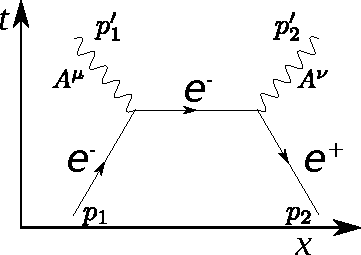
\includegraphics[scale=0.6]{qhu}
  \caption{Un doblete de quarks, $Q$, ingresa con su hipercarga de $\color{red}1/6$ al vértice denotado por el {\color{OliveGreen}punto verde}, y junto con un doblete de Higgs de hipercarga $\color{blue}1/2$ generan un quark up derecho, $u_R$ de hipercarga $2/3$. La ecuación resultante para la conservación de hipercarga en la parte superior derecha de la figura, es compatible con el término en el Lagrangiano una vez se reemplaza la hipercarga negativa por el campo conjugado, $\left( u_R \right)^{\dagger}$. }
  \label{fig:yg}
\end{figure}

Como en mecánica cuántica todos los procesos que mantienen la conservación de la carga tienen alguna probabilidad de ocurrir, entonces los diagramas que construyamos con algún flujo consistente de alguna carga conservada, serán automáticamente permitidos por la teoría. El cálculo explícito de la probabilidad se realiza haciendo la expansión de la denominada matriz $S$ en teoría cuántica de campos.

Por lo tanto, podemos construir diagramas de flujo de cargas conservadas para explorar las predicciones de un Lagrangiano  a nivel cualitativo. 

\section{Masas de neutrinos}
Si introducimos un neutrino derecho, $N_R$, con número leptónico $-1$,  al  modelo estándar, se genera al menos la contribución de Dirac
\begin{align}
  \underbrace{\mathcal{L}_{\text{Dirac}}}_{\displaystyle Y:}=
  \underbrace{h  \epsilon_{ab} L^{a} H^{b} \left( N_R \right)^{\dagger}}_{\displaystyle L+H -N_R=0 } +\text{h.c}\,. 
\end{align}
La ecuación de conservación de hipercarga es representada en la figura~\ref{fig:lhn}\footnote{Por lo tanto en el operador de Weinberg todos los campos entran al vértice efectivo}

\begin{figure}
  \centering
  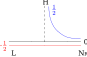
\includegraphics[scale=0.6]{lhn}
  \caption{Un doblete de leptones, $L$, ingresa con su hipercarga de $\color{red}-1/2$ al vértice  y junto con un doblete de Higgs de hipercarga $\color{blue}1/2$ generan un  neutrino derecho, $N_R$, de hipercarga $0$. }
  \label{fig:lhn}
\end{figure}



\section{Masas de neutrinos a 1-loop}
Contenido de partículas
  \begin{align*}
  R_{d}=&
  \begin{pmatrix}
    \psi_{L}^{0}\\
    \psi_{L}^{-}
  \end{pmatrix}
&  
\widetilde{R}_{u}=&
  \begin{pmatrix}
   - \left( \psi_{R}^{-} \right)^{\dagger}\\
     \left(\psi_{R}^{0}\right)^{\dagger}
  \end{pmatrix},
\end{align*}



\begin{table}
  \centering
  \begin{tabular}{|l|l|l|l|}
    \hline  
    Symbol     & $\left( SU(2)_L, U(1)_Y \right)$ & $Z_2$ & \text{Spin}\\ \hline
    $S_{\alpha}$ & $(1,0)$ & $-$ & 0\\
    $\left( N_R \right)^{\dagger}$  & $(1,0)$ & $-$ & 1/2\\
     $\widetilde{R}_u$, & $(2, +1/2)$ & $-$ & 1/2\\ 
     $R_d$ & $(2, -1/2)$ & $-$ & 1/2\\ \hline
  \end{tabular}
  \caption{Conjunto $\alpha$ de escalares y fermiones de Weyk del modelo.}
  \label{tab:partcont}
\end{table}

El correspondiente Lagrangiano incluye los siguientes términos con las correspondientes ecuaciones para la conservación de la hipercarga
\begin{align}
\label{eq:lt13a}
  \underbrace{\mathcal{L}}_{\displaystyle Y:}
=
  &
 \underbrace{M_D \epsilon_{ab}R^a_d \widetilde{R}^b_u}_{\displaystyle R_d-R_u=0}
    - \underbrace{\tfrac{1}{2}M_N  N_RN_R}_{\displaystyle N_R+N_R=0}
    -\underbrace{h_{i\alpha} \epsilon_{ab}\widetilde{R}_u^a L_{i}^b S_{\alpha}}_{\displaystyle -R_u+L+S=0}
    -\underbrace{\lambda_d\, \epsilon_{ab}H^a R_d^b \left( N_R \right)^{\dagger}}_{\displaystyle  H+ R_d- N_R=0}
    -\underbrace{\lambda_u \epsilon_{ab}\widetilde{H}^a \widetilde{R}_u^b \left( N_R \right)^{\dagger}}_{\displaystyle H-R_u-N_R=0}
    \nonumber\\
&+\text{h.c}
\end{align}

Con estos campos e interacciones podemos construir el diagrama de masas de neutrinos a 1-loop que se ilustra en la figura~\ref{fig:lhlh}.

\begin{figure}
  \centering
  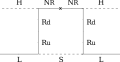
\includegraphics[scale=0.6]{lhlh}
  \caption{Masas de neutrinos a 1-loop para el Lagrangiano~\eqref{eq:lt13a} }
  \label{fig:lhlh}
\end{figure}

Note que el diagrama directo con $R_u$ no es compatible con un Higgs entrando al vértice, como exige la figura~\ref{fig:lhn}. Por lo tanto es inconsistente con masas de neutrinos. Finalmente, si asociamos un número leptónico de $-1$ a todos los campos fermiónicos de la figura~\ref{fig:lhlh}, entonces el término $N_R N_R$ termina violando el número leptónico en dos unidades. 

%%% Local Variables: 
%%% mode: latex
%%% TeX-master: "fullnotes"
%%% ispell-local-dictionary: "castellano8"
%%% End: 
